\chapter{Results: Online Sources}\chlbl{online_sources}
%
\begin{figure}[h]
    \centering
    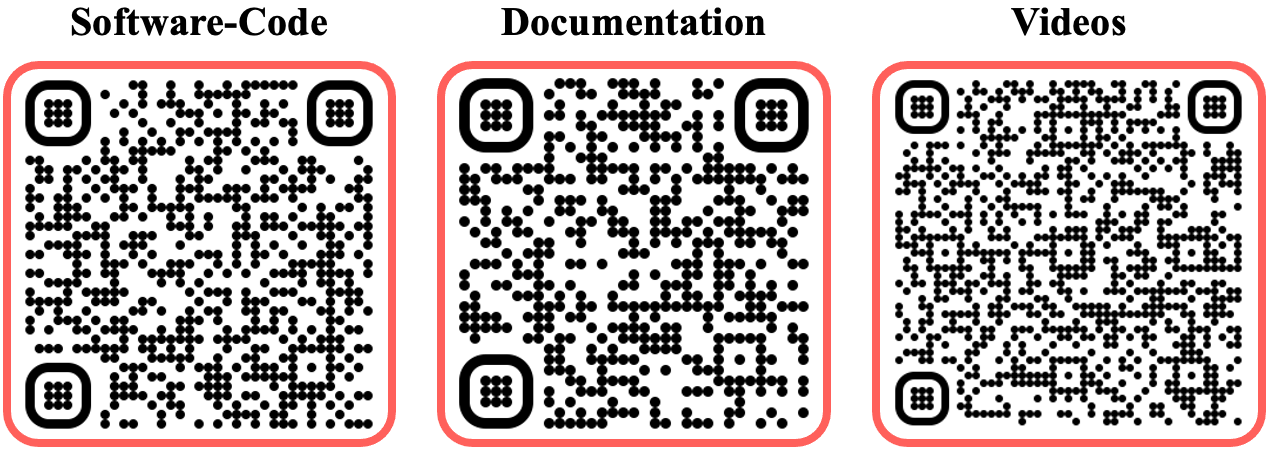
\includegraphics[width=0.79\textwidth]{qr_links}
    \caption[QR-Codes with links to sources]{QR-Codes with links to sources. The first code directs to the GitHub repository containing the source code, the second code to the repository containing the \LaTeX-files to build this documentation, and the third code points to video visualisations of the results.}
    \figlbl{qr_links}
\end{figure}
%
The codebase and results from this thesis have been released as open source on GitHub: The code is available at \href{https://github.com/sagerpascal/lateral-connections}{github.com/sagerpascal/lateral-connections}, and the documentation is available at \href{https://github.com/sagerpascal/msc-thesis}{github.com/sagerpascal\\/msc-thesis}.
Furthermore, a GitHub webpage provides video visualisations from some of the results is available at \href{https://sagerpascal.github.io/lateral-connections/results/final_results.html}{sagerpascal.github.io/lateral-connections/results/final\_results}.
QR codes linking to these URLs are provided in \figref{qr_links} for convenient access using electronic devices.


\section{Video}\seclbl{result_video}
%
\begin{figure}[h]
    \centering
    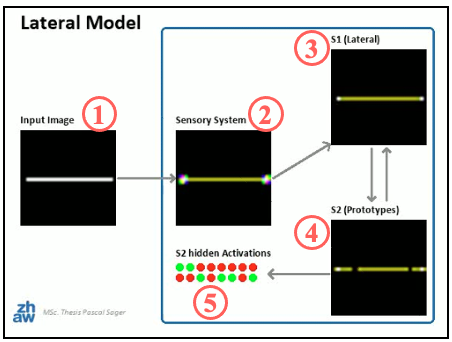
\includegraphics[width=0.89\textwidth]{video_overview}
    \caption[Overview of components visualised in the videos]{An overview of the components visualised in the videos.}
    \figlbl{video_overview}
\end{figure}
%
In the following, the video visualisations accessible at \href{https://sagerpascal.github.io/lateral-connections/results/final_results.html}{sagerpascal.github.io\\/lateral-connections/results/final\_results} are explained.
These explanations are limited to an overview of which components are shown in each video.
An interpretation of the video contents is provided in the corresponding result section.

Two video versions are shown for each experiment, both produced by the same model using the same parameter weights.
In the first video version, the Bernoulli neuron is replaced by a neuron using a fixed threshold.
This provides a video output that is more stable and has no flickering activations caused by sampling from a probability distribution.
For the \emph{S0} and \emph{S1} stages, a threshold of $0.5$ is used. Consequently, neurons with a probability of $\geq 0.5$ are set to $1$, while the other neurons are set to $0$.
A threshold of $0.9$ is used for the \emph{S2} stage, visualising only activities with high certainty that roughly correspond to those accepted by \emph{S1} as feedback signals.
The second video shows the network activities when the Bernoulli neurons are used.

Each video visualises the processing of the input over time.
The first six video frames show how the video is processed over $T=6$ timesteps of the fast loop, followed by five additional frames depicting the final prediction after the fast loop.
By doing so, viewers have time to analyse the network's activations during this short interruption before the next input is fed into the model, and the process repeats.

In \figref{video_overview}, a single video frame is shown, providing an overview of the components displayed in each video:
\begin{enumerate}
    \item The left part of the video displays the input image fed into the sensory system. It is a binary image with one colour channel, whereby active pixels are depicted in white and inactive pixels are depicted in black.
    \item The activations of the sensory system \emph{S0} are shown in the middle of the video. The sensory system extracts $4$ features at each location. Each feature combination is visualised in a different colour, and areas without activations are depicted in black.
    \item \emph{S1} is visualised in the top right corner. It uses the same colours as the sensory system. However, the activations might differ since neurons with insufficient lateral support are turned off, or other neurons might switch on.
    \item \emph{S2} is shown in the bottom right corner. It uses the same colours as the sensory system and \emph{L1}. The visualisation depicts the returned prototype, i.e., the feedback provided to \emph{S1} after mapping \emph{S1}' activities to the latent variables.
    \item The latent variables of \emph{S2} are shown at the center bottom of the video as $16$ circles. Each circle represents a cell, with green indicating an active cell and red indicating an inactive one. 
\end{enumerate}

For a detailed explanation of the content and observations in each video, please refer to the results chapter of this thesis.

\chapter{Negative Hebbian Learning}\chlbl{neg_hebb_updates}
%
\begin{figure}[h]
    \centering
    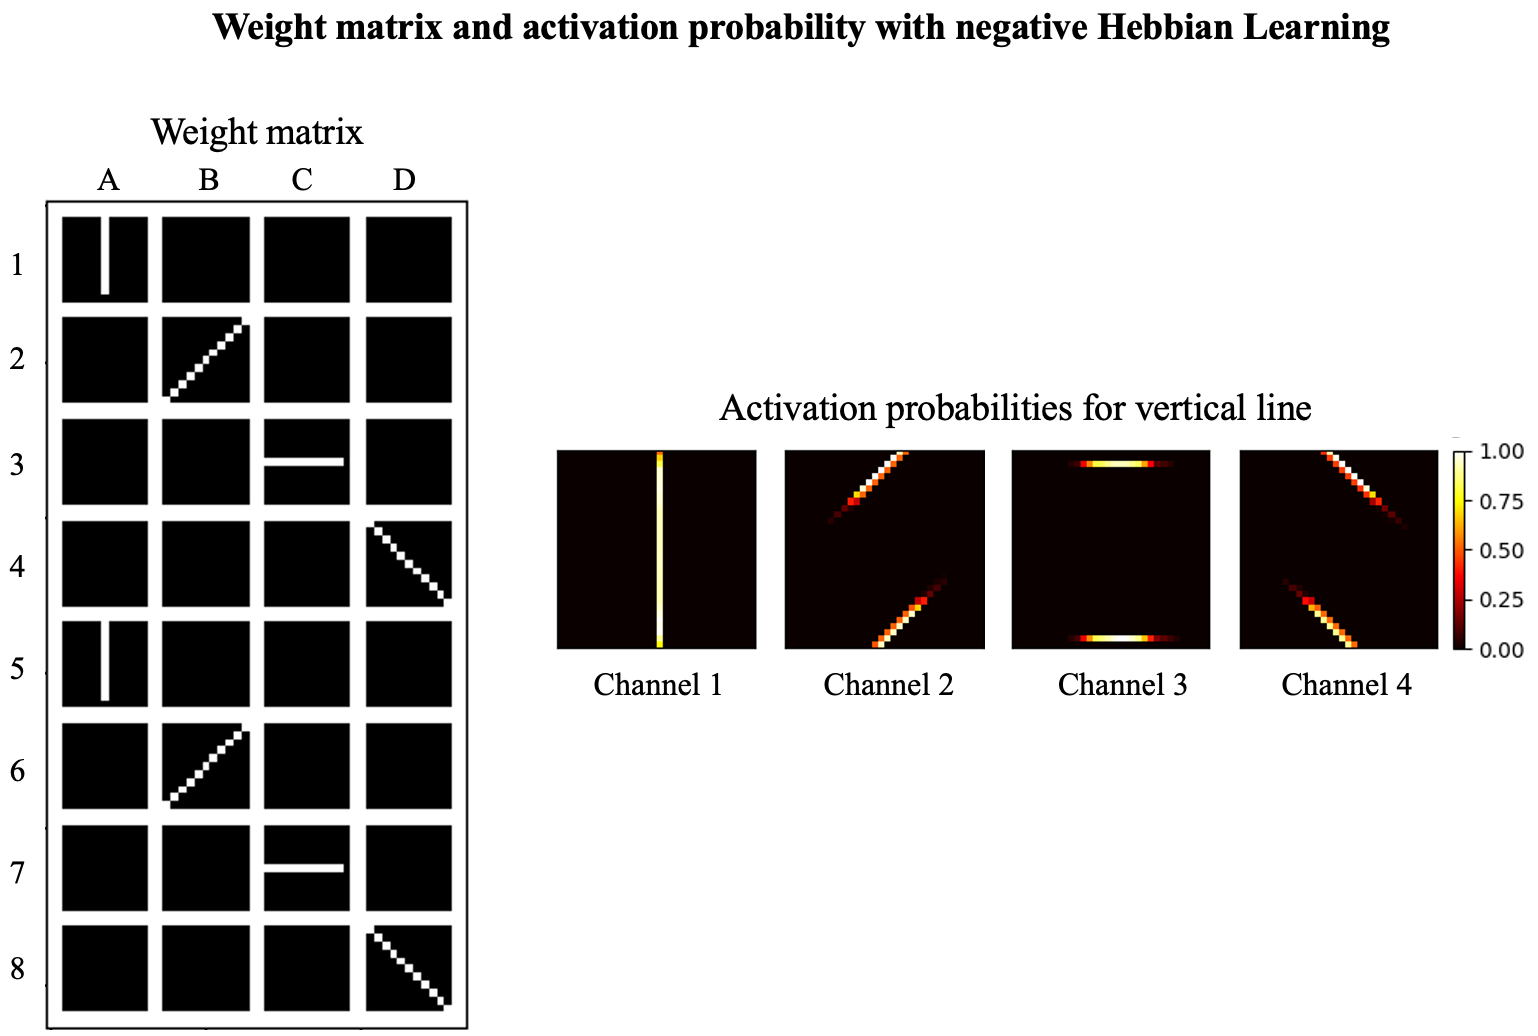
\includegraphics[width=0.99\textwidth]{neg_hebb_learning}
    \caption[Weight matrix and activations with negative Hebbian learning]{The weight matrix and the corresponding activation probabilities for a vertical line of a model trained with negative Hebbian learning.}
    \figlbl{neg_hebb_learning}
\end{figure}
%
In this section, the concept of negative Hebbian Learning in \emph{S1} is examined, a learning paradigm designed to allow neural networks to forget unimportant or inconsistent features. 
In the conducted experiments, only positive Hebbian learning \sidecite{hebb_organization_1949} is used to strengthen connections between active cells.
Conversely, negative Hebbian learning additionally reduces the connection strength between cells that fire disjointly\sidenote{I.e. one cell is active while the other is inactive.}.
While negative Hebbian learning facilitates eliminating previously learned but inconsistent connections, it also poses challenges in maintaining desired lateral connections that are needed to provide support between feature cells.


In \figref{neg_hebb_learning}, the weight matrix of a model trained with negative Hebbian updates and the activation probabilities of a vertical line fed into the model is visualised.
Despite the divergence of the activation probabilities compared to those of positive Hebbian learning (c.f. \figref{S1_weight_analysis}), these activations are still considered valid representations of lines.
However, the major issue is that the output channels do not rely on multiple distinct features.

For instance, the output channel $A$ representing vertical lines only considers the input channels $1$ and $5$, whereby channel $1$ contains the ``vertical lines features'' from the sensory system, and channel $5$ is its own recurrent connection.
Regrettably, input channels $2$-$4$, which contain additional sensory signals, are disregarded by output channel $A$. Therefore, only cells representing vertical line features support this output channel.
In contrast, positive Hebbian learning considers all input channels, resulting in different features supporting each other.

Consequently, negative Hebbian learning leads to lower lateral support within the network.
This might not be an issue for the used line dataset but is crucial for real-world scenarios\sidenote{For example, one channel could represent eyes and another channel eyelashes. These features should support each other.}.
Negative Hebbian learning, while facilitating the filtering out of irrelevant features, also tends to make features mutually exclusive, which prevents learning adequate support between them.

\begin{figure}[h]
    \centering
    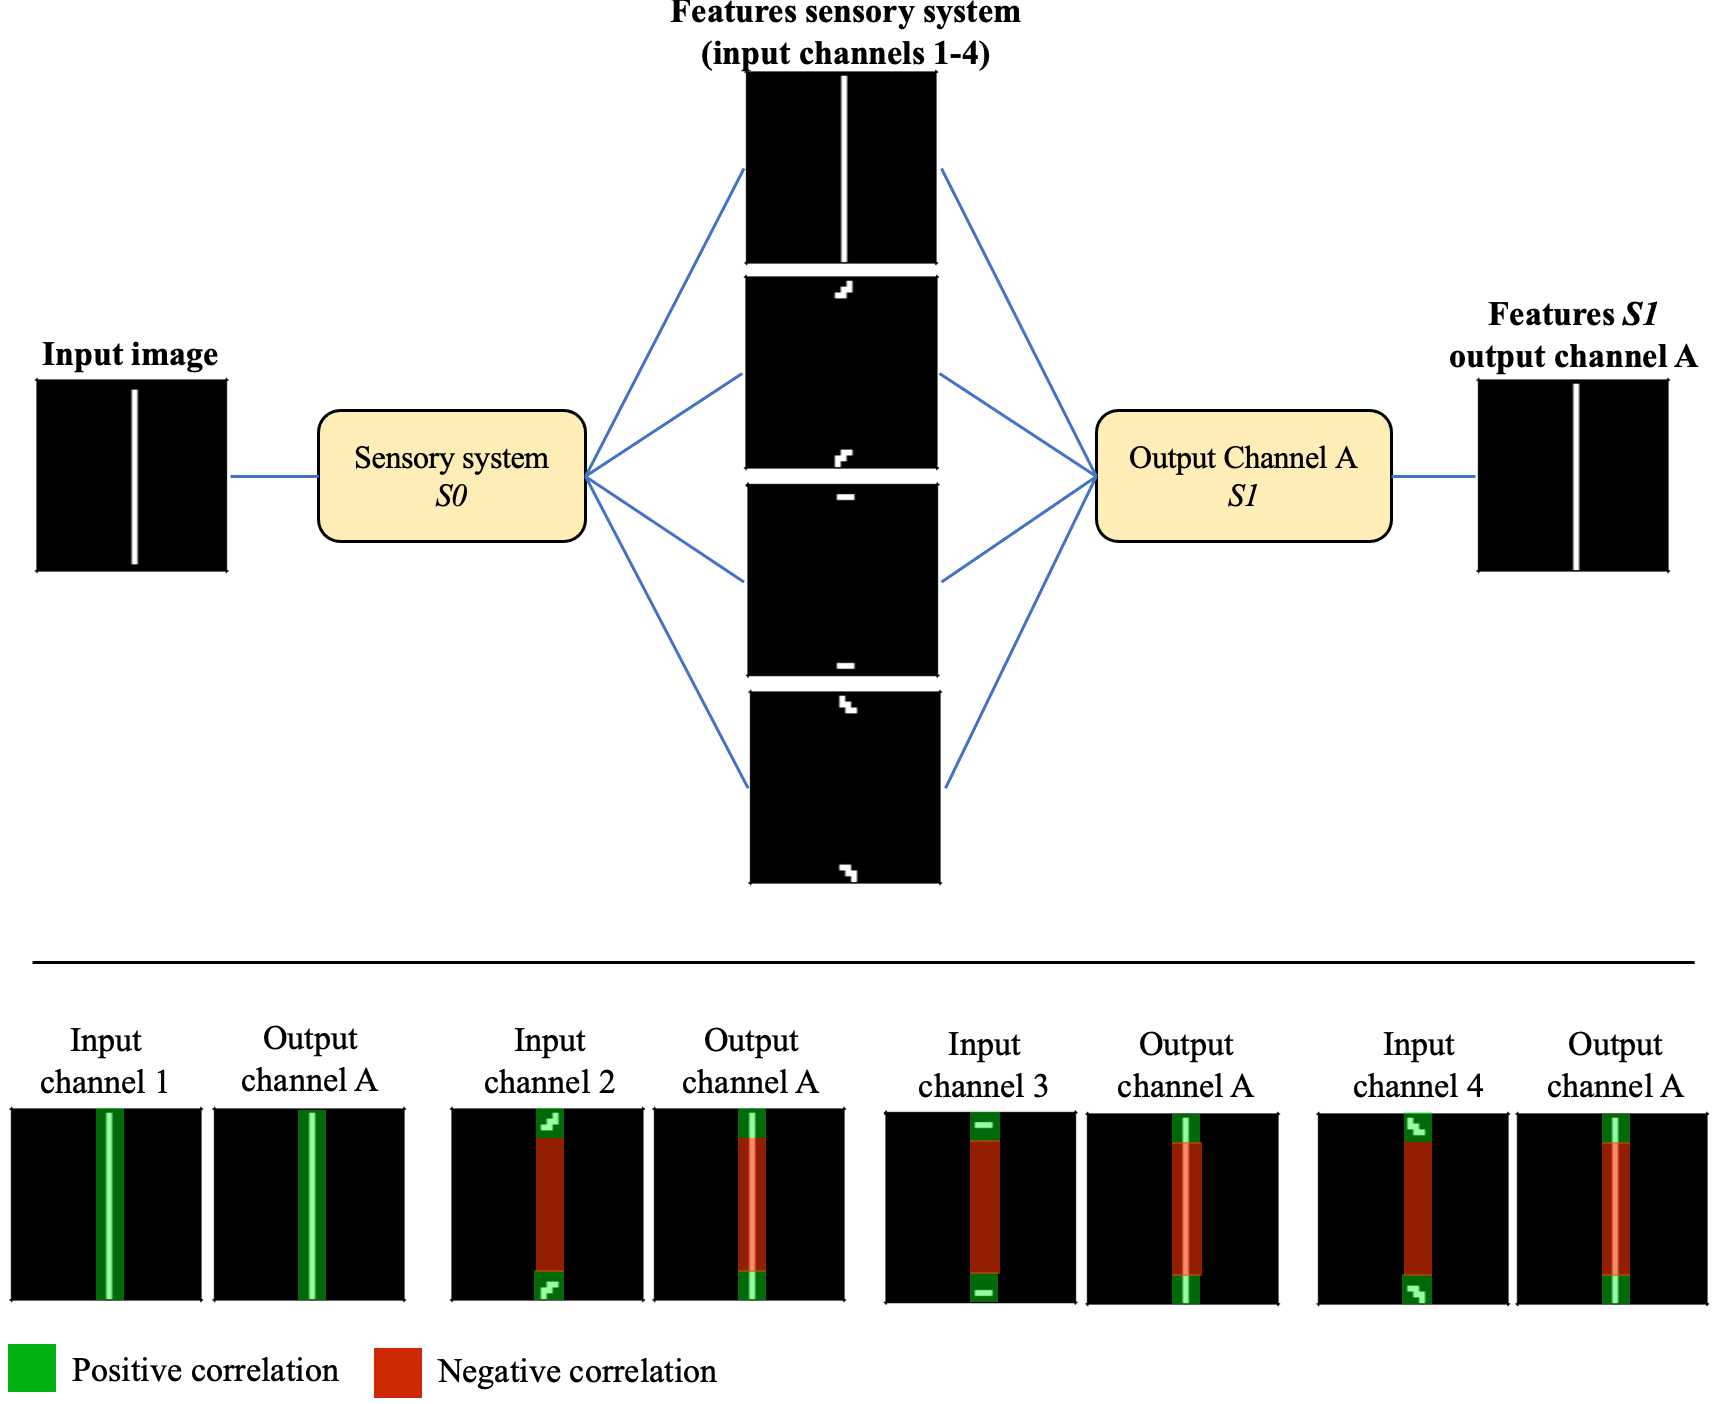
\includegraphics[width=0.99\textwidth]{correlations_hebb_learning}
    \caption[Feature correlation analysis]{Correlation between features from sensory input channels and the output channel $A$. The upper part of the images visualises the sensory features fed into output channel $A$ and the expected result. The lower part of the image indicates where positive and negative correlation occurs between sensory channels and output channel $A$.}
    \figlbl{correlations_hebb_learning}
\end{figure}
%
The primary issue is that, except for one input channel, there are more negative correlations between the input channels and a single output channel, as illustrated in \figref{correlations_hebb_learning}.
In this context, ``negative correlation'' refers to disjointly active cells, while ``positive correlation'' refers to cells that fire together.
In the case of the vertical line, the output channel $A$ is expected to reassemble the line roughly.

Hebbian learning compares this output with the input channels, strengthening the weights for positively correlated input-output pairs and weakening them for negatively correlated pairs.
These correlations are visualised in the lower part of \figref{correlations_hebb_learning}.
Input channel $1$ and output channel $A$ have high similarity. Therefore, the activations between input and output have a positive correlation, and the corresponding lateral connections defined by kernel $A1$ undergo a positive Hebbian update.
However, all the other channels have a positive correlation only at the line ends and a negative correlation in the middle section of the line.
Consequently, there is more negative than positive correlation at the kernels $A2$-$A4$, and these features undergo more negative than positive updates.
This causes the lateral support learned at the line ends to be suppressed by the negative updates.

The resolution to this issue remains unclear and requires additional experiments. One potential approach is to use a significantly lower learning rate for negative updates than for positive updates; another solution could be to introduce alternative cells (c.f. \secref{future_alt_cells})

